
\documentclass{beamer}
\usetheme[faculty=ped]{fibeamer}

\usepackage[utf8]{inputenc}
\usepackage[
main=english,
czech, slovak 
]{babel} 

\title{Aplicație Web pentru prezentarea și vânzarea de miere online}
\subtitle{ESTIC 2023} 
\author{Tudor Vlăduț-Alexandru}

\makeatletter
\renewcommand\fibeamer@includeLogo[1][]{}
\makeatother

\usepackage{ragged2e}  % `\justifying` text
\usepackage{booktabs}  % Tables
\usepackage{tabularx}
\usepackage{tikz}      % Diagrams
\usetikzlibrary{calc, shapes, backgrounds}
\usepackage{amsmath, amssymb}
\usepackage{url}       % `\url`s
\usepackage{listings}  % Code listings
\frenchspacing
\begin{document}
	\shorthandoff{-}
	\frame[c]{\maketitle}
	
	\begin{darkframes}
		\begin{frame}<beamer>
			\frametitle{Cuprins}
			\tableofcontents
		\end{frame}
		
		\section{Introducere}
		\subsection{Ce este aplicația mea web?}
		\begin{frame}[label=lists]{Introducere}
			\framesubtitle{Ce este aplicația mea web?}
			\begin{columns}[onlytextwidth]
				\column{0.5\textwidth}
				\begin{itemize}
					\item Ecommerce Website - magazin online cu miere
				\end{itemize}
				
				\column{0.5\textwidth}
				 \begin{figure}
					\centering
					
\includegraphics[width=0.6\textwidth]{logo.png}
				\end{figure}
			\end{columns}
		\end{frame}
		
		

		\subsection{Tehnologii folosite}
		\begin{frame}[label=lists]{Introducere}
			\framesubtitle{Ce tehnologii am folosit?}
			\begin{columns}[onlytextwidth]
				\column{1\textwidth}
				\begin{itemize}
					\item HTML - limbaj de marcare
					\item CSS - limbaj de stilizare
					\item JavaScipt - limbaj de scripting
					\item JSON - format de reprezentare a datelor
					\item Firebase - o bază de date NoSQL
				\end{itemize}
			\end{columns}
			
		\end{frame}
		
		
		\section{Ce cuprinde aplicația web?}
		
		
		\begin{frame}[label=math]{Ce cuprinde aplicația web?}
			\vspace{-1em}
			\framesubtitle{1/6}
			\begin{columns}[t]
				\begin{column}{1\textwidth}
					\begin{exampleblock}{Pagina principală}
					    \tiny
						Unde se găsesc \alert{informațiile necesare}.
						\begin{itemize}
							\item Este structurată în așa fel încât să găsești tot ce ai nevoie: informații despre noi, despre produsele disponibile, o galerie foto, unde ne localizăm etc.
							\item Design și export din Nicepage, iar unele elemente sunt editate în Photoshop
							\item Pentru afișarea unei hărți cu locația am folosit Google Maps Embed API
						\end{itemize}
					\end{exampleblock}
					\vspace{-1em}
					\begin{figure}
						\centering
						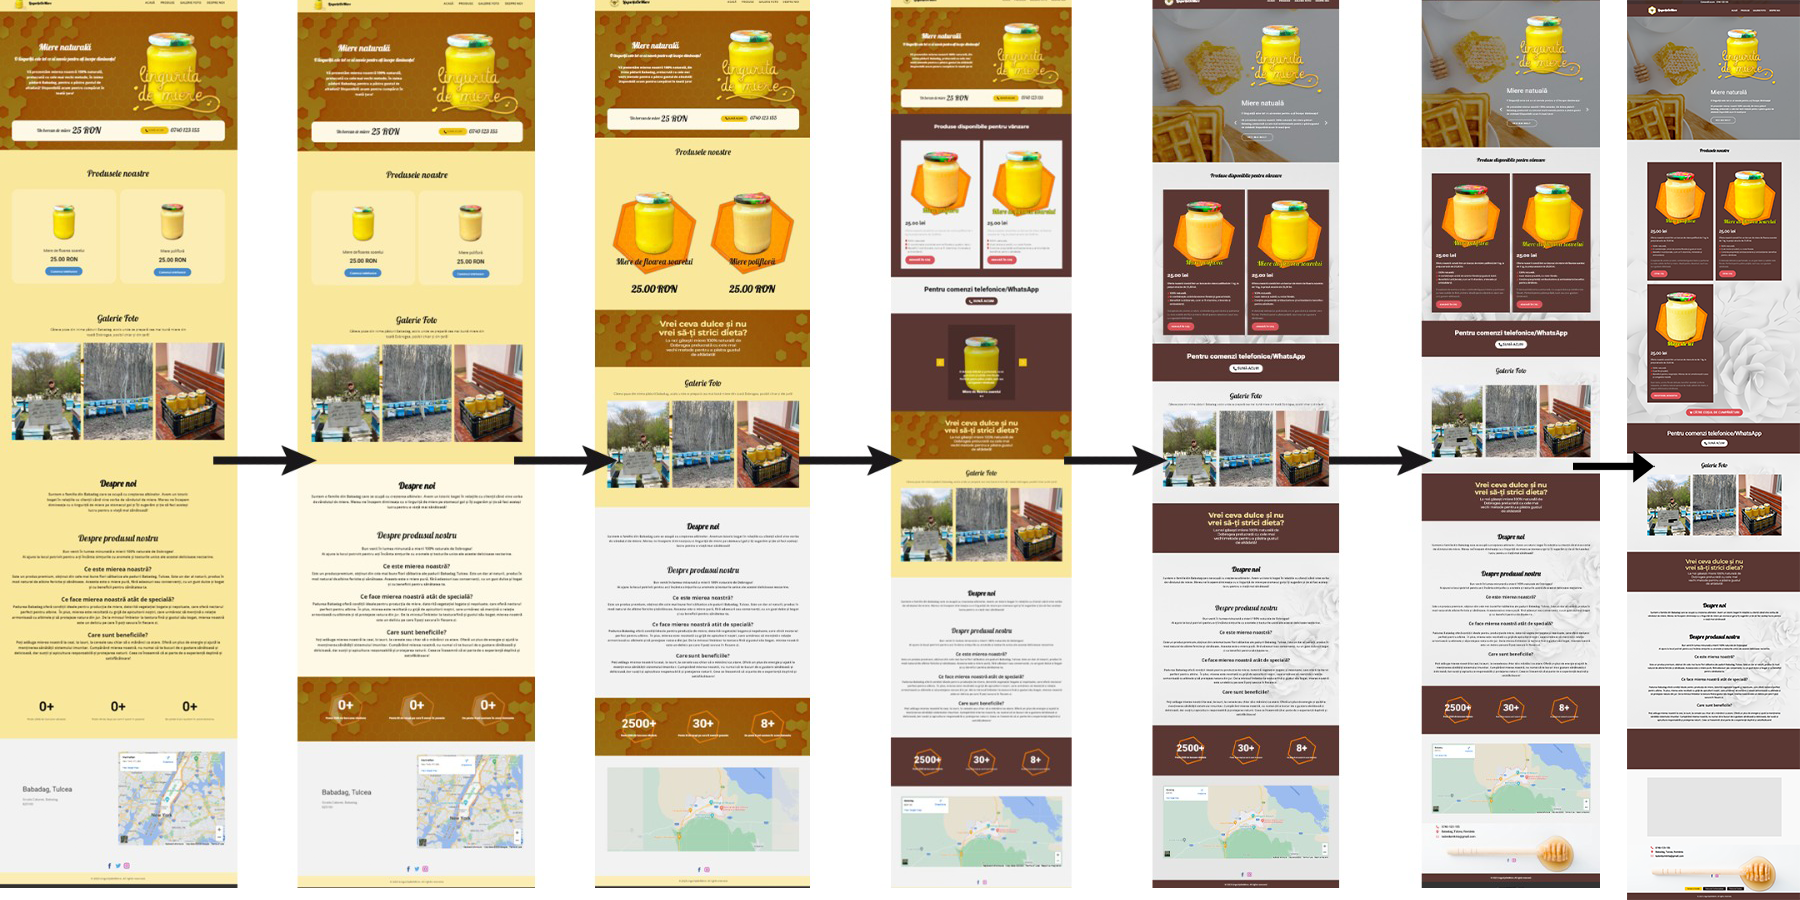
\includegraphics[width=0.8\textwidth]{evolutie.png}
					\end{figure}
				\end{column}
			\end{columns}
		\end{frame}
		
		\begin{frame}[label=math]{Ce cuprinde aplicația web?}
			\vspace{-1em}
			\framesubtitle{2/6}
			\begin{columns}[t]
				\begin{column}{1\textwidth}
					\begin{exampleblock}{Pagina cu recenzii}
						\tiny
						Unde toată lumea poate \alert{evalua site-ul și produsele și poate posta comentarii}.
						\begin{itemize}
							\item Nu necesită logarea utilizatorului , toată lumea poate să posteze o recenzie
							\item Validatoare: toate câmpurile trebuie completate, limbaj-ul vulgar este verificat printr-un JSON cu cuvinte inadecvate
							\item Informațiile se stochează în baza de date Firebase
						\end{itemize}
					\end{exampleblock}
					\vspace{-1em}
					\begin{figure}[!tbp]
						\centering
						\begin{minipage}[b]{0.29\textwidth}
							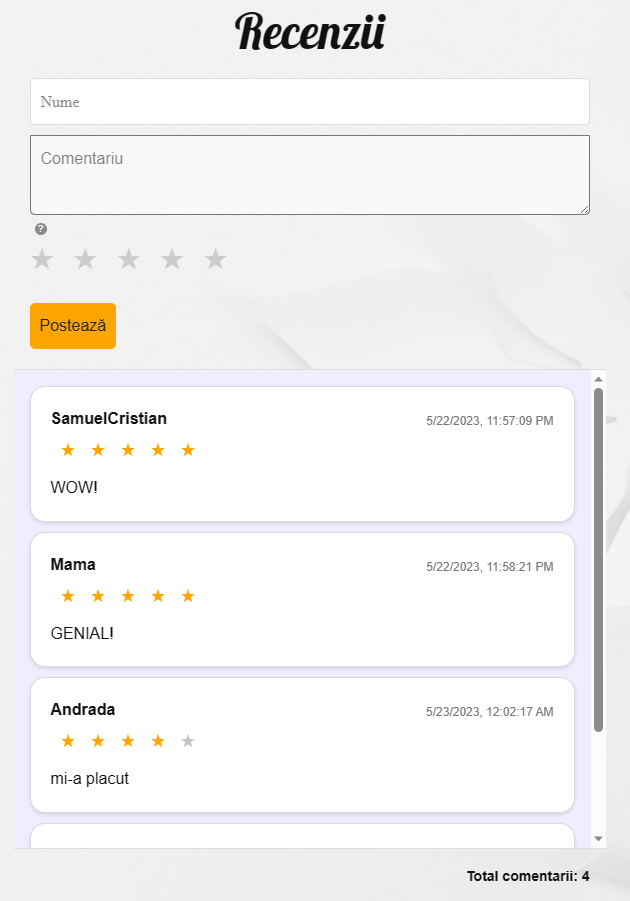
\includegraphics[width=\textwidth]{recenzii.png}
						\end{minipage}
						\hfill
						\begin{minipage}[b]{0.69\textwidth}
							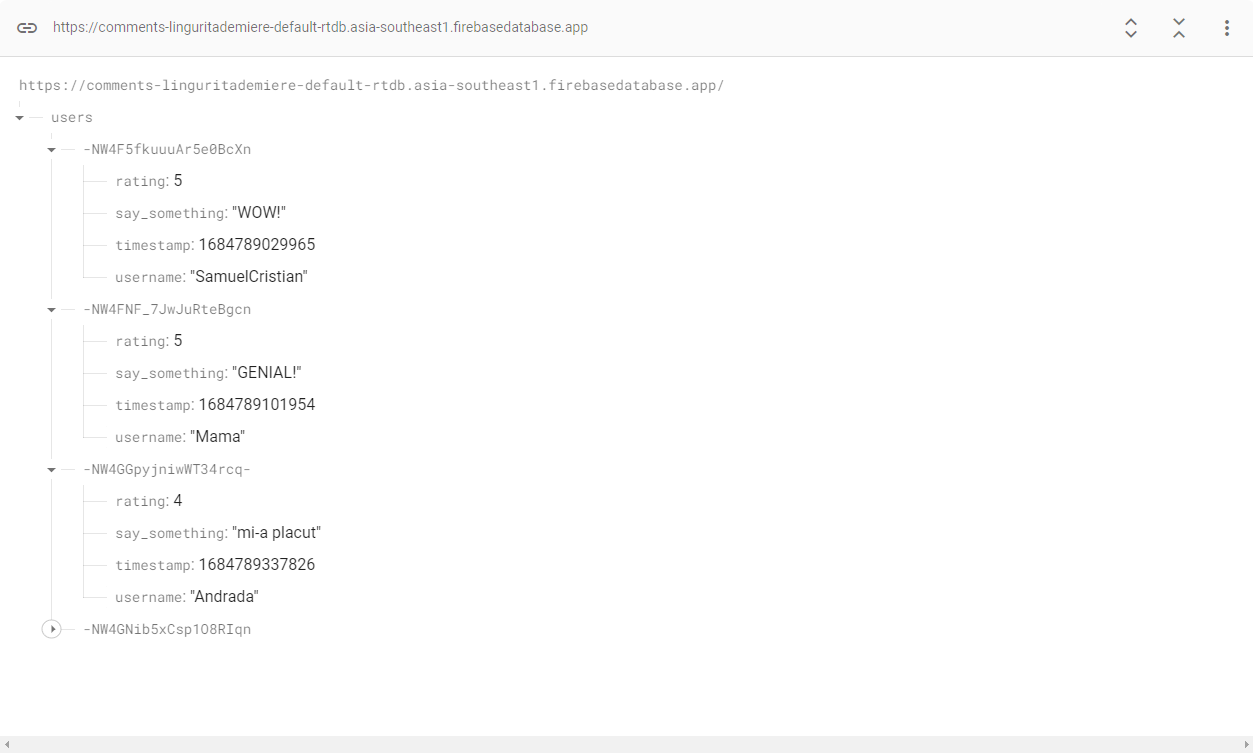
\includegraphics[width=\textwidth]{firebase.png}
						\end{minipage}
					\end{figure}
				\end{column}
			\end{columns}
		\end{frame}
		
		\defverbatim[colored]\sleepSort{
			\begin{lstlisting}[language = C,tabsize=2]
		for each cuvant_vulgar in cuvinte_vulgare do
			for each cuvant_din_comentariu in cuvinte_din_comentariu do
				if cuvant_din_comentariu contains cuvant_vulgar then
					DisplayAlert("The comment uses offensive language.")
					SetAlertColor("red")
					return
				end if
			end for
		end for
		\end{lstlisting}}
	
		\defverbatim[colored]\sleepSortt{
			\begin{lstlisting}[language = C,tabsize=2]
				for each i from 0 to length(stars) do:
					if i < rating then
						set stars[i] as highlighted
					else
						set stars[i] as not highlighted
				
		\end{lstlisting}}
		
		\begin{frame}{Algoritm pentru verificarea cuvintelor vulgare}
			\sleepSort
			\begin{minipage}[t]{1\textwidth}
				\centering
				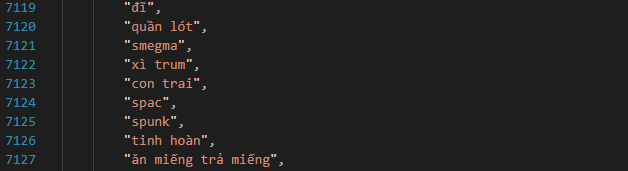
\includegraphics[width=\textwidth]{json.png}
			\end{minipage}
		\end{frame}
		
		\begin{frame}[c]{Algoritm pentru gestionarea evidențierii stelelor de rating}
			\vspace{-2em}
			\sleepSortt
			\begin{center}
				\vspace{2em}
				\begin{minipage}[t]{0.5\textwidth}
					\centering
					
\includegraphics[width=\textwidth]{stele.png}
				\end{minipage}
			\end{center}
		\end{frame}
		
		\begin{frame}[label=math]{Ce cuprinde aplicația web?}
			\vspace{-3em}
			\framesubtitle{3/6}
			\begin{columns}[t]
				\begin{column}{1\textwidth}
					\begin{exampleblock}{Pagina cu informații suplimentare}
						\tiny
						Unde găsești \alert{mai multe informații} despre noi și despre produse.
						\begin{itemize}
							\item Un grafic cu vânzările anuale, făcut cu Chart.js
							\item Generator de imagini în funcție de ce buton apeși, implementat cu Unsplash API
						\end{itemize}
					\end{exampleblock}
					\vspace{1em}
					\begin{center}
						\begin{minipage}[t]{0.49\textwidth}
							\centering
							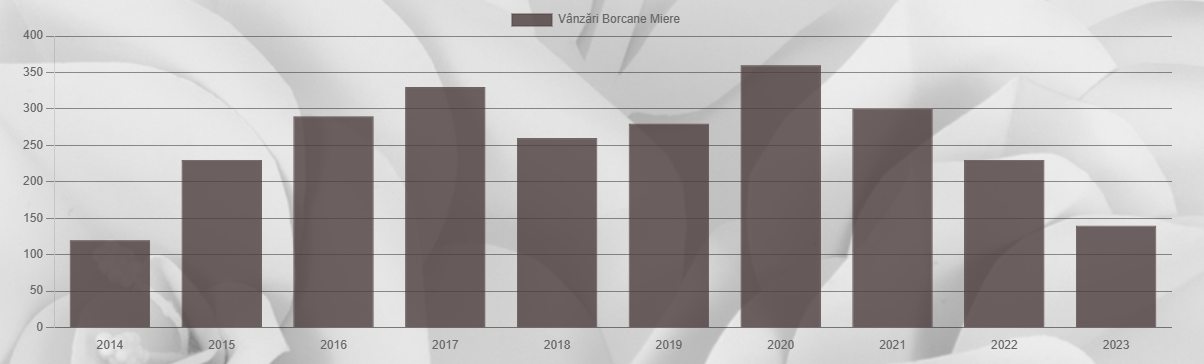
\includegraphics[width=\textwidth]{grafic.png}
						\end{minipage}
						\hfill
						\begin{minipage}[t]{0.49\textwidth}
							\centering
							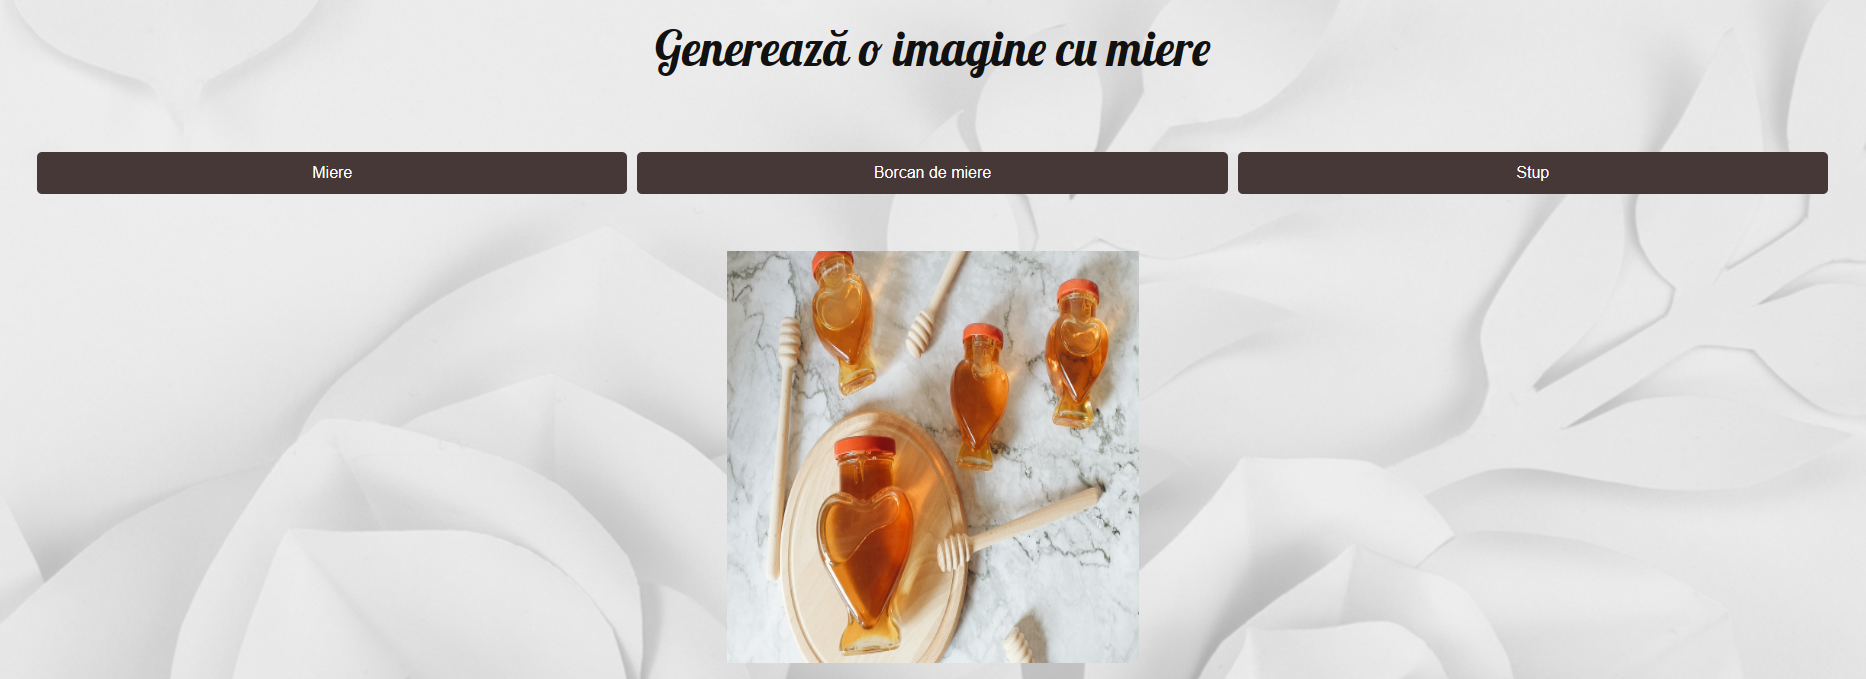
\includegraphics[width=\textwidth]{generator.png}
						\end{minipage}
						
						\vspace{0.5em}
						
						\begin{minipage}[t]{0.6\textwidth}
							\centering
							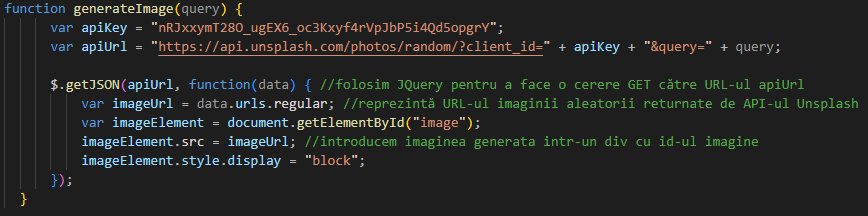
\includegraphics[width=\textwidth]{codgenerator.png}
						\end{minipage}
					\end{center}
				\end{column}
			\end{columns}
		\end{frame}
		
		
		
		\begin{frame}[label=math]{Ce cuprinde aplicația web?}
			\vspace{-1em}
			\framesubtitle{4/6}
			\begin{columns}[t]
				\begin{column}{1\textwidth}
					\begin{exampleblock}{Pagini cu: termeni și condiții, politică de cookies și politică de confidențialitate}
						\tiny Unde utilizatorii pot găsi informații despre \alert{termeni, condiții, livrare, comandă, politică de cookies și de confidențialitate etc.}
					\end{exampleblock}
					\begin{exampleblock}{Pagina unde te redirecționează după ce trimiți comanda}
						\tiny Unde se \alert{confirmă trimiterea comenzii}, iar utilizatorii pot vedea informațiile trimise de ei.
						\begin{itemize}
							\item Tot cu Unsplash API se generează o imagine cu miere în momentul când intri pe pagină 
						\end{itemize}
					\end{exampleblock}
					\vspace{-1em}
					\begin{center}
						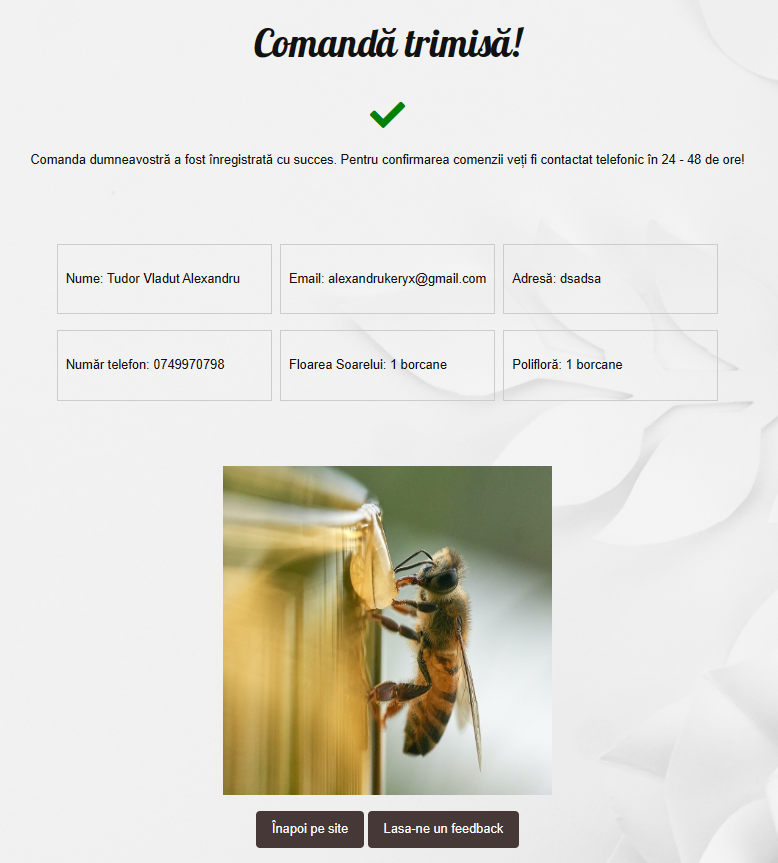
\includegraphics[width=0.25\textwidth]{comandatrimisa.png}
					\end{center}
				\end{column}
			\end{columns}
		\end{frame}
		
		\begin{frame}[label=math]{Ce cuprinde aplicația web?}
			\vspace{-1em}
			\framesubtitle{5/6}
			\begin{columns}[t]
				\begin{column}{1\textwidth}
					\begin{exampleblock}{Pagina cu coșul de cumpărături}
						\tiny
						Unde utilizatorul poate \alert{trimite comenzi.}
						\begin{itemize}
							\item \alert{Validatoare}: toate câmpurile trebuie completate, coșul să nu fie gol, prețurile să nu fie negative, să bifezi termenii și condițiile, să introduci o valoare valida pentru câte borcane cumperi, email-ul să fie cu @ și numărul de telefon să fie de 10 cifre; la numărul de telefon și codul poștal poți să introduci doar cifre
							\item Detaliile comenzii sunt trimise prin \alert{formsubmit.co}. În caz de pică serverele, există un buton în josul paginii de unde se poate trimite mail
							\item Iconițe implementate cu librăria \alert{Font Awesome}, iar detaliile utilizatorului și coșul de cumpărături sunt stocate în browser prin \alert{sessionStorage}
							\item Prin manipulări ale DOM-ului și \alert{calcule matematice} simple, am implementat următorii \alert{algoritmi}: incrementarea și decrementarea cantității până la maximum 30 de produse, calcularea subtotalului în funcție de cantitatea și prețul produselor, actualizarea prețului total în funcție de livrare și subtotal
						\end{itemize}
					\end{exampleblock}
					\vspace{-1em}
					\begin{figure}[!tbp]
						\centering
						\begin{minipage}[b]{0.45\textwidth}
							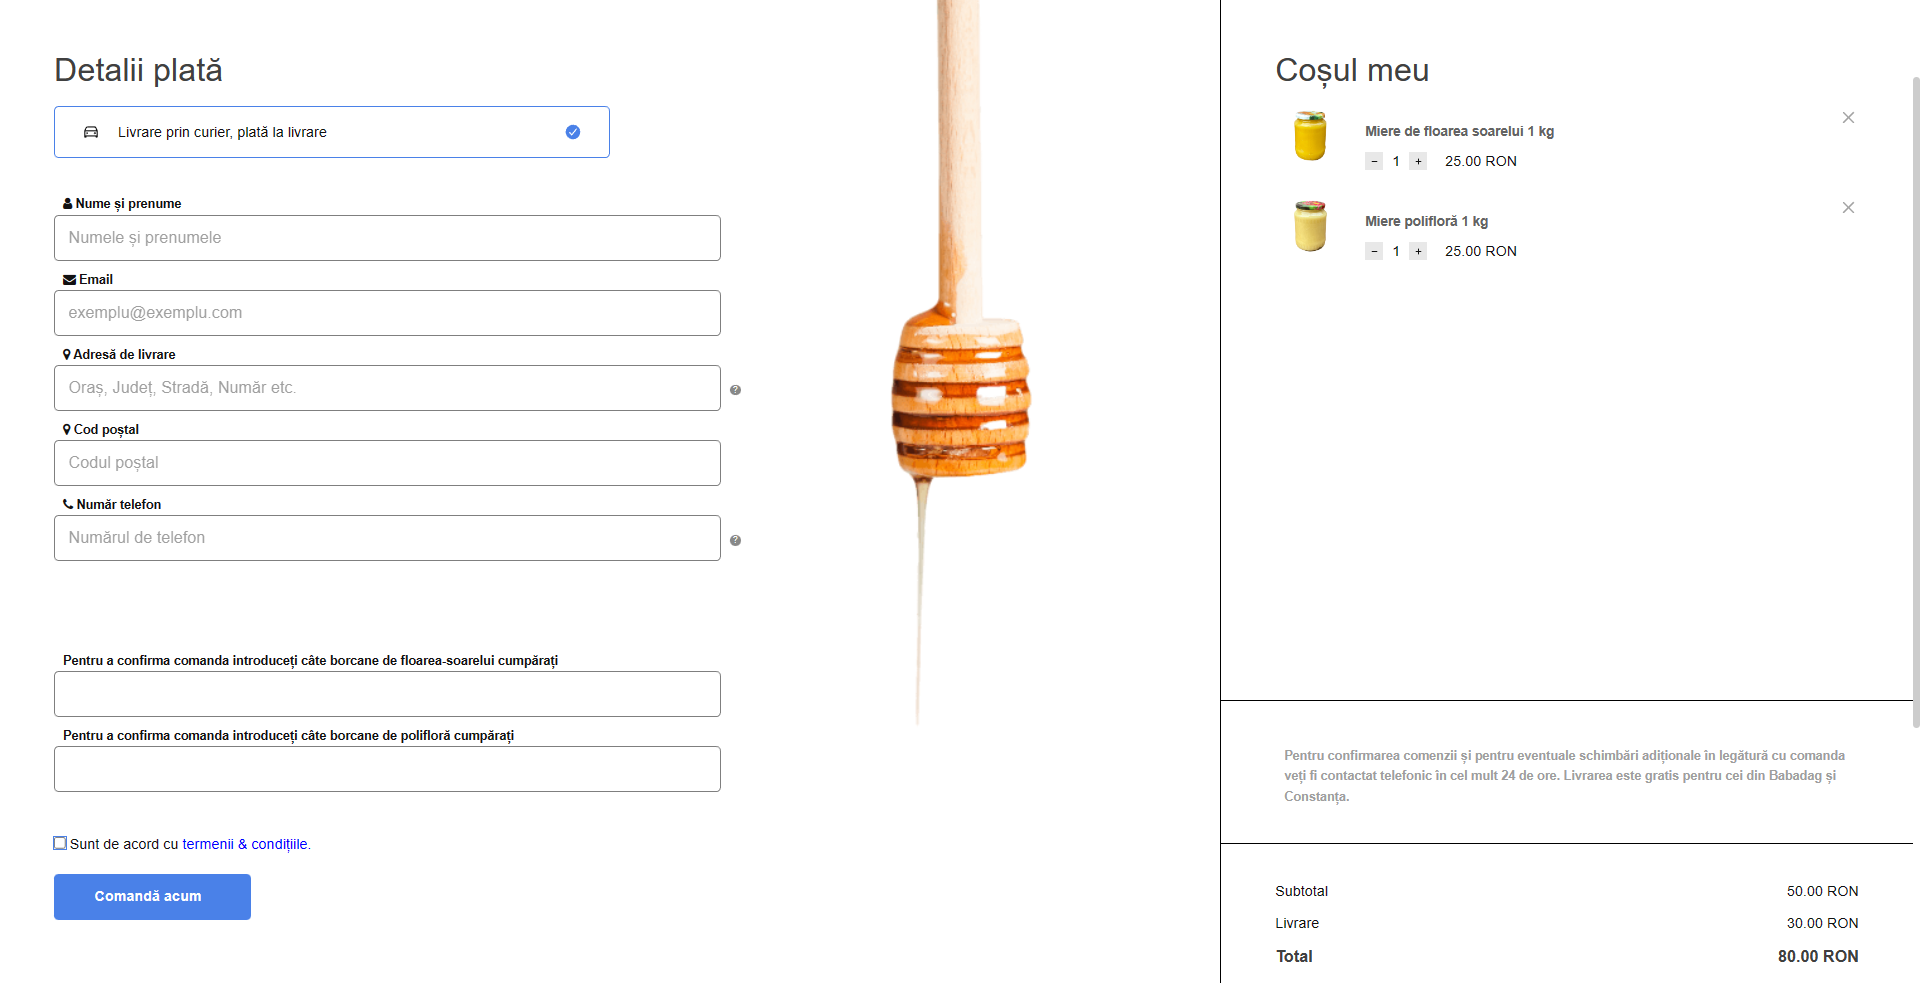
\includegraphics[width=\textwidth]{shop.png}
						\end{minipage}
						\hfill
					\end{figure}
				\end{column}
			\end{columns}
		\end{frame}
		
		\begin{frame}[label=math]{Ce cuprinde aplicația web?}
			\vspace{-1em}
			\framesubtitle{6/6}
			\begin{columns}[t]
				\begin{column}{1\textwidth}
					\begin{exampleblock}{O implementare Google Analytics}
						\tiny
						Unde pot vedea \alert{toate statisticile despre interactiunea utilizatorilor cu website-ul.}
					\end{exampleblock}
					\vspace{0em}
					\begin{figure}[!tbp]
						\centering
						\begin{minipage}[t]{0.7\textwidth}
							\centering
							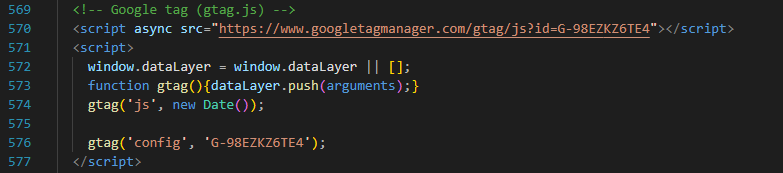
\includegraphics[width=\textwidth]{codgoogle.png}
						\end{minipage}
						\hfill
						
						\vspace{0.5em}
						
						\begin{minipage}[t]{0.7\textwidth}
							\centering
							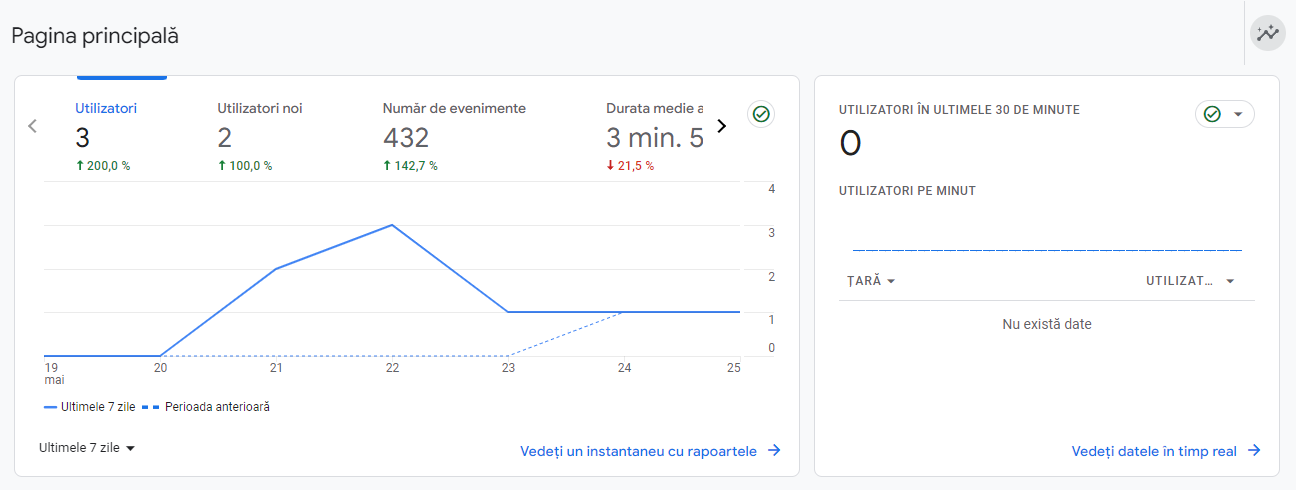
\includegraphics[width=\textwidth]{google.png}
						\end{minipage}
						\hfill
					\end{figure}
				\end{column}
			\end{columns}
		\end{frame}
		
		\section{Ce urmează să implementez pe viitor?}
		
		\begin{frame}{Ce urmează să implementez pe viitor?}
			\framesubtitle{1/2}
			\begin{itemize}
				\item Să implementez Google Ads
				\item Plata cu cardul - stripe.com
				\item Utilizatorul să se poată abona la Newsletter, astfel primește promoții pe mail ,coduri de reducere și anunțuri
				\item Să mă documentez în legătură cu regulile pentru un shop online, să fie totul legal, să îl hostez , să cumpăr SSL și domain 
				\item Să-i mai fac debugging, să aranjez mai bine codul , să trec prin HTML validator și CSS validator
				\item Să se elimine informația din sessionStorage în momentul în care comanda este trimisă 
			\end{itemize}
		\end{frame}
		
		\begin{frame}{Ce urmează să implementez pe viitor?}
			\framesubtitle{2/2}
			\begin{itemize}
				\item Să fac funcționalitatea shop-ului mai generală:
			\end{itemize}
			\vspace{1em}
			\begin{center}
				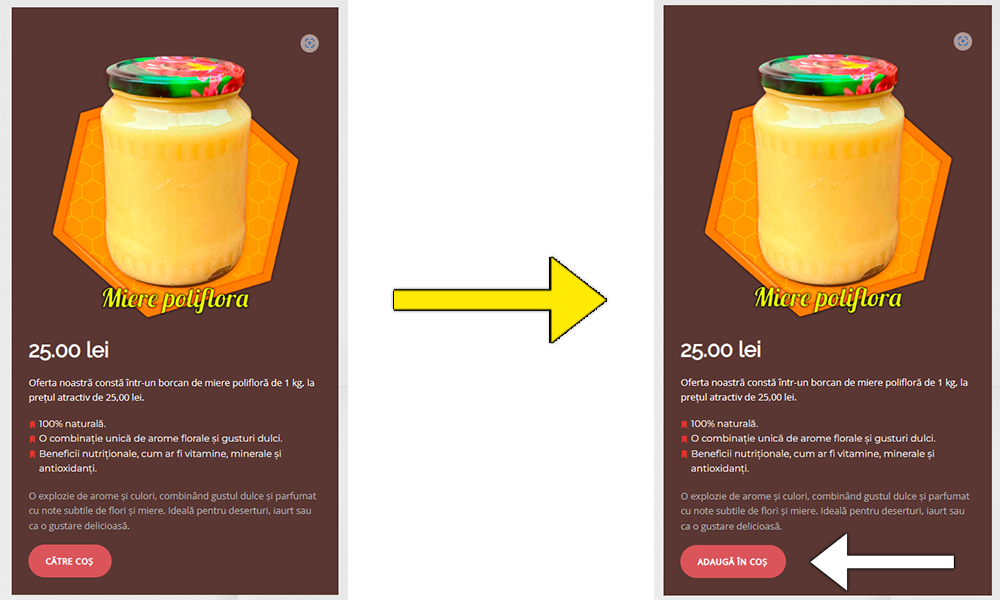
\includegraphics[width=0.9\textwidth]{PRODUSSSSSS.png}
			\end{center}
		\end{frame}
		
		
		\section{Concluzie}
		
		\begin{frame}[label=citations]{Concluzie}
			
			\justifying\ Aplicația noastră web pentru prezentarea și vânzarea de miere oferă o platformă simplă și eficientă pentru a conecta consumatorii pasionați de miere cu produsele noastre excepționale. Cu un design elegant și o navigare simplă, aplicația noastră creează o experiență plăcută și ușor de utilizat pentru clienți.
		\end{frame}
		
		\section{Bibliografie}
		
		\begin{frame}[label=bibliography]{Bibliografie}
			\begin{thebibliography}{9}
				
				\bibitem{honeybenefits}
				\emph{Healthline: The Benefits of Honey}.
				Disponibil pe \url{http://www.healthline.com/nutrition/10-benefits-of-honey}.
				
				\bibitem{javascriptbook}
				Rob Percival, Maaike van Putten, Laurence Lars Svekis.
				
				\emph{JavaScript from Beginner to Professional}.
				Publisher, 2021.
				
				\bibitem{miere}
				\emph{Informatii despre miere}.
				Disponibil pe \url{https://aurumnoblehoney.com/miere-dulce-sanatoasa/informatii-despre-miere/}.
				
				\bibitem{javascriptmdn}
				\emph{MDN Web Docs: JavaScript}.
				Disponibil pe \url{https://developer.mozilla.org/en-US/docs/Web/JavaScript}.
				
				\bibitem{javascriptw3schools}
				\emph{W3Schools: JavaScript Tutorial}.
				Disponibil pe \url{https://www.w3schools.com/js/}.
				
		\end{thebibliography}		
		\end{frame}
		
	\end{darkframes}
\end{document}